\section{Datenbank}\label{sec:Realisierung-Datenbank}

Die Realisierung des Datenbank-Schemas wird über Migrationen in der Komponente des Game Information Systems durchgeführt. Sie wird jedoch aus Verständnisgründen in diesem Kapitel erläutert.

Die im Entwurf (\autoref{sec:Entwurf-Datenbank}) vorgestellten Tabellen wurden ohne Anpassungen realisiert. Da die Punkteberechnung nicht im Game Information System durchgeführt werden soll, werden Views in der Datenbank genutzt, welche die benötigten Daten aus den verschieden Tabellen zusammensetzen.

Eine SQL-Datei zur Erstellung des Datenbank-Schemas befindet sich auf dem mit abgegebenen Datenträger der Bachelorarbeit, wurde aber aus Platzgründen weder hier, noch im Anhang aufgenommen.

\subsection{Punkteübersicht}
Die Folgenden Views wurden in der Datenbank erstellt, um die Punkteberechnung zu ermöglichen. Sie wurde kleinschrittig gehalten, um eine Nachvollziehbarkeit zu gewährleisten.

\subsubsection{Angriffspunkte}\label{subsubsec:Angriffspunkte}
\begin{center}
	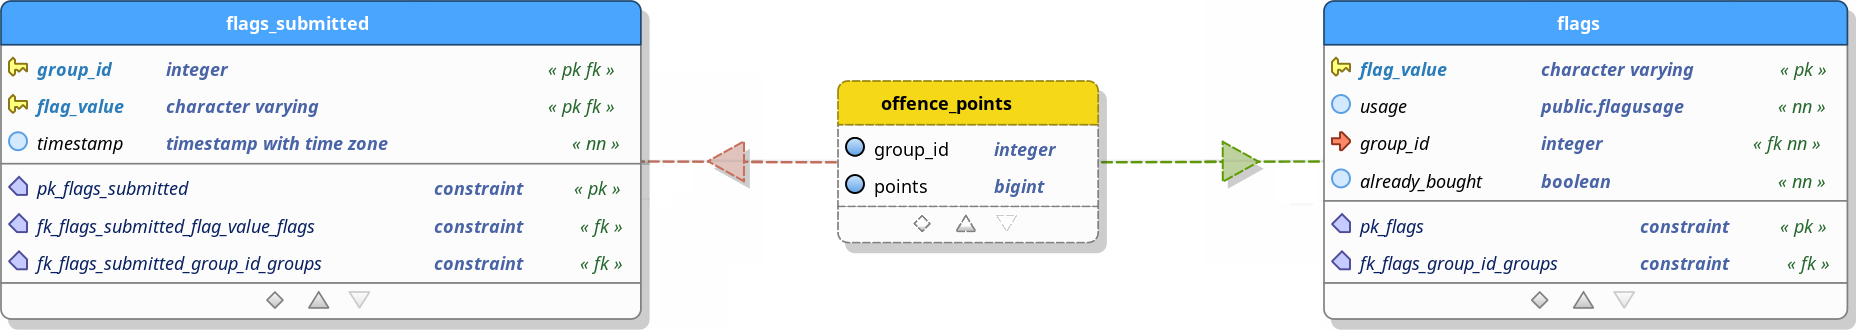
\includegraphics[width=\linewidth]{realisierung/database/view-offence}
	\captionof{figure}{View Angriffspunkte (ER-Diagramm)}
	\label{fig:realisierung-view-offence}
\end{center}

Wie in \autoref{fig:realisierung-view-offence} erkennbar werden die Angriffspunkte (\textit{offence\_points}) über die Tabellen \textit{flags} und \textit{flags\_submitted} berechnet. Dies erfolgt, indem alle abgegebenen Flags mit den im Spiel vorhanden Flags verbunden werden (\textit{JOIN}), um nur Flags zu beachten, die von einer anderen Gruppe als der Besitzenden abgegeben wurden. Im Anschluss werden diese pro Gruppe gezählt und als Offensivpunkte ausgewiesen.

\begin{lstlisting}[frame=single, language=sql, caption={SQL View Angriffspunkte}, captionpos=b, label={lst:database-offence-points}]
SELECT flags_submitted.group_id, count(flags_submitted.flag_value) AS points
FROM (flags_submitted JOIN flags ON (((flags_submitted.flag_value)::text = (flags.flag_value)::text)))
WHERE (flags_submitted.group_id <> flags.group_id)
GROUP BY flags_submitted.group_id;
\end{lstlisting}

\subsubsection{Defensivpunkte}
Ähnlich den Angriffspunkten (\ref{subsubsec:Angriffspunkte}) werden die Defensivpunkte (Strafe für verlorene Flags) berechnet.
Anders als bei den Angriffspunkten werden alle vorhanden Flags mit den abgegebenen Flags für jede Gruppe gejoint, wenn die besitzende Gruppe ungleich der abgebenden Gruppe ist. In dieser Liste können Flags mehrfach auftreten, wenn mehrere Gruppen einer Gruppe Flags gestohlen haben. Da im alten System ein Verlust einer Flag an mehrere Gruppen nur einmal mit Minuspunkten bestraft worden ist, werden in der Liste der Flags mit der SQL Klausel \textit{DISTINCT} Duplikate entfernt. Im Anschluss werden dann die verlorenen Flags pro Gruppe gezählt und so die Defensivpunkte bestimmt.

\begin{lstlisting}[frame=single, language=sql, caption={SQL View Denfensivpunkte}, captionpos=b, label={lst:database-defence-points}]
SELECT flags.group_id, count(DISTINCT flags.flag_value) AS points
FROM (flags JOIN flags_submitted ON (((flags.flag_value)::text = (flags_submitted.flag_value)::text)))
WHERE (flags.group_id <> flags_submitted.group_id)
GROUP BY flags.group_id;
\end{lstlisting}

\subsubsection{Erkundungspunkte}
Die Erkundungspunkte werden nach dem gleichen Vorgehen wie die Angriffspunkte (\ref{subsubsec:Angriffspunkte}) bestimmt. Einziger Unterschied ist, dass nur Flags beachtet werden, bei denen die besitzende Gruppe gleicher der abgebenden Gruppe ist.

\begin{lstlisting}[frame=single, language=sql, caption={SQL View Erkundungspunkte}, captionpos=b, label={lst:database-discover-points}]
SELECT flags_submitted.group_id, count(flags_submitted.flag_value) AS points
FROM (flags_submitted JOIN flags ON (((flags_submitted.flag_value)::text = (flags.flag_value)::text)))
WHERE (flags_submitted.group_id = flags.group_id)
GROUP BY flags_submitted.group_id;
\end{lstlisting}

\subsubsection{Strafpunkte}
Die View der Strafpunkte (\textit{penalty\_points}) summiert die in der \textit{penalties}-Tabelle vorhandenen Strafpunkte pro Gruppe. Andere Informationen wie Grund der Strafe bleiben hierbei unberücksichtigt. Jede Gruppe (\textit{group\_id}) hat entsprechende Strafpunkte (\textit{total\_penalty}). Sollte eine Gruppe bisher noch keine Strafpunkte erhalten haben, wird diese in der View nicht aufgeführt.

\subsubsection{Servicepunkte}
In der View \textit{group\_service\_points} werden pro Gruppe pro Service die Servicepunkte sowie die Serviceprozentzahl berechnet. Dazu werden Daten aus den Tabellen \textit{services} und \textit{group\_service\_status} benötigt. Aus der Tabelle \textit{services} wird einzig die Gewichtung der einzelnen Services abgefragt. In der Tabelle \textit{group\_service\_status} werden die Anzahl der durchgeführten sowie der erfolgreichen Scans pro Gruppe abgerufen.

Die Servicepunkte diene als Leistungsindikator der Absicherung und der Instandhaltung des Systems durch die Studierenden. Dazu wird von der Anzahl der erfolgreichen Scans die Anzahl aller Scans abgezogen und das Ergebnis der Subtraktion gewichtet, um einen geringeren Einfluss auf die Gesamtpunkte zu ermöglichen.

\begin{equation*}
	\frac{Anzahl~erfolgreicher~Scanvorgaenge - Anzahl~Scanvorgaenge}{Gewichtung}=~Strafpunkte
\end{equation*}


Die Serviceprozentzahl stellt für die Studierenden und für betreuenden Personen die prozentuale Erreichbarkeit dar. Für die Berechnung dieser Prozentzahl pro Gruppe und Service wird die folgende Formel verwendet: 

\begin{equation*}
	\frac{100}{Anzahl~erfolgreicher~Scanvorgaenge}~*~Anzahl~Scanvorgaenge~=~Wert~in~\%
\end{equation*}

Um das Ergebnis einer Division durch 0 zu verhindern, wird im SQL Quelltext die Funktion \textit{COALESCE} verwendet. Diese nimmt den ersten Wert ungleich Null. Bei der Punkteberechnung kann durch eine Gewichtung von 0 die Division ein Ergebnis von Null zurückgeben. Deshalb wird dann die Gewichtung standardmäßig auf eins gesetzt. Wenn eine Gruppe keine erfolgreichen Scanvorgänge zu vermelden hat, wird das Ergebnis der Formel für die Serviceprozentzahl auf 0 gesetzt.

\begin{lstlisting}[frame=single, language=sql, caption={SQL Abfang von Division durch 0}, captionpos=b, label={lst:database-service-points-divison-by-0}]
COALESCE(NULLIF((services.weight)::integer, 0), 1)

COALESCE(((100 / group_service_status.scan_count) * group_service_status.online_count), 0)
\end{lstlisting}

\subsubsection{Flagshoppunkte}
Bei den Flagshoppunkten handelt es sich, um die für Käufe ausgegebenen Punkte einer Gruppe.
Für die Berechnung wird die Summe der Kosten aller gekauften Pakete pro Gruppe gebildet.
Wenn eine Gruppe keine Ausgaben getätigt hat, wird diese auch nicht in die View aufgenommen.

\subsubsection{Challengepunkte}
Im Gegensatz zum alten Überwachungs- und Auswertungssystems wird der Start einer Challenge nicht länger mit Minuspunkten bestraft. Diese Minuspunkte bewirken meiner Meinung nach eine Abschreckung der Studierenden, sodass diese die Challenges nicht versuchen. Im Rahmen einer Lehrveranstaltung sollten die Studierenden ermutigt werden, verschiedene themenbezogene Aufgaben zu lösen.

Die Challengepunkte werden mithilfe der Tabellen \textit{challenges} und \textit{group\_has\_challenges} in der View \textit{challenge\_points} bestimmt. Für jede Gruppe werden die Punkte der gelösten Challenges summiert.

Sollten Negativpunkte für gestartete Challenges verteilt werden, muss der SQL Code der View angepasst werden, damit für jede gestartete Challenge Negativpunkte verrechnet werden. 

\subsubsection{Gesamtpunkte}
\begin{center}
	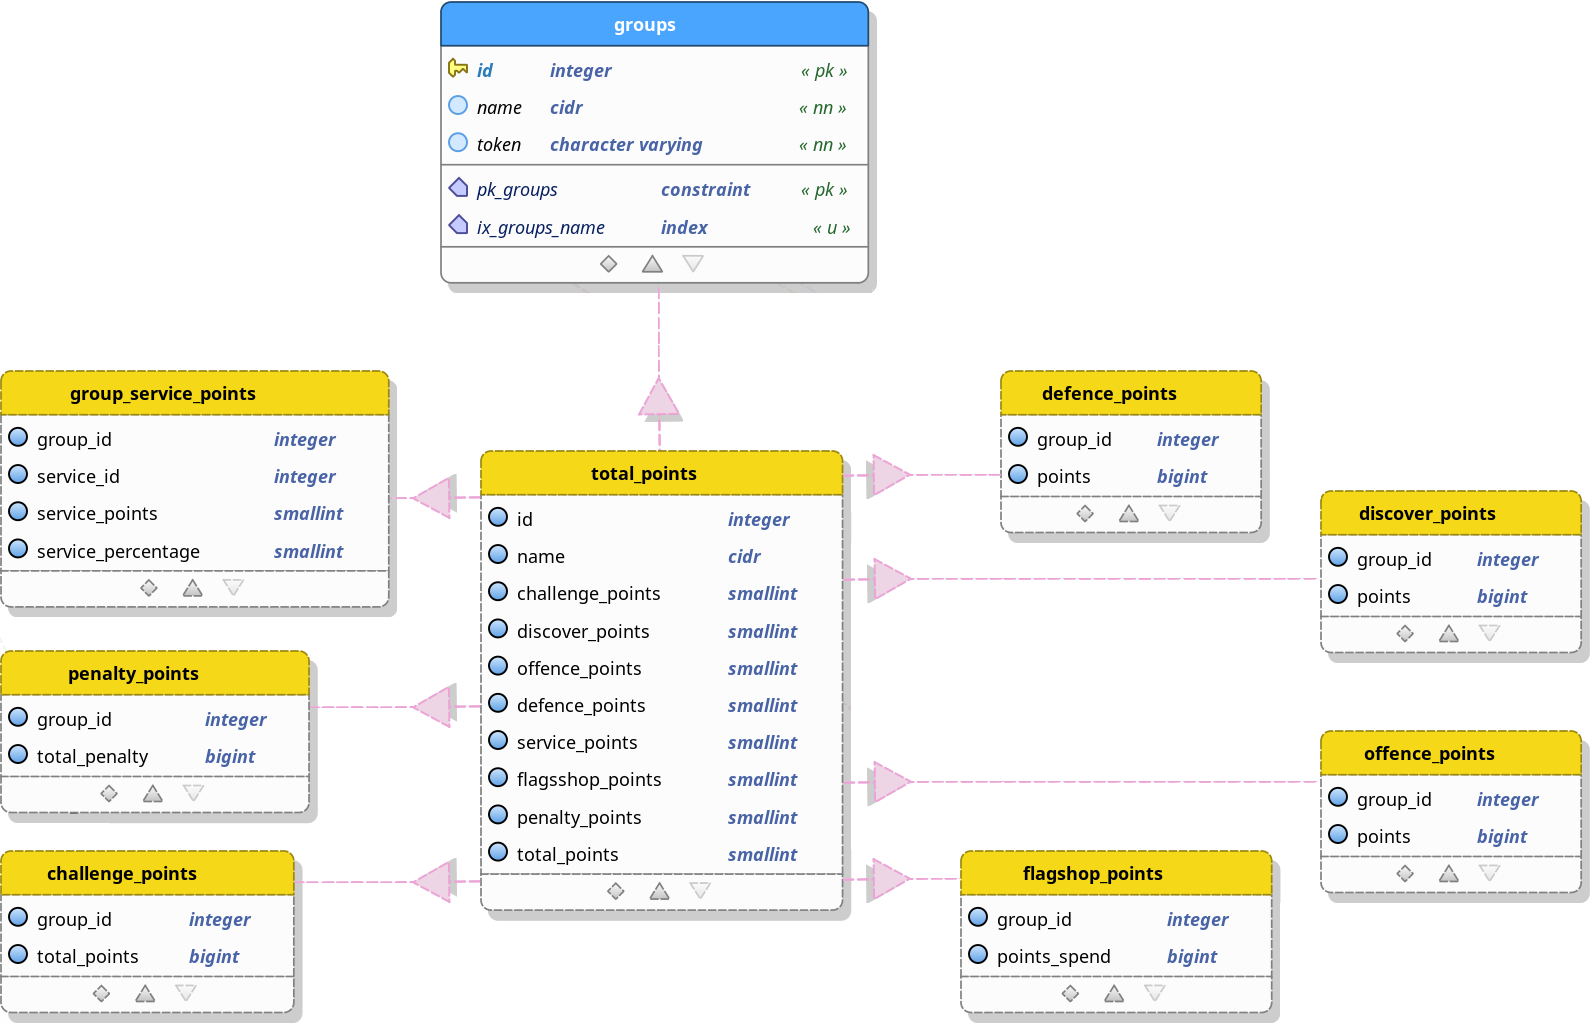
\includegraphics[width=\linewidth]{realisierung/database/view-total}
	\captionof{figure}{View Gesamtpunkte (ER-Diagramm)}
	\label{fig:realisierung-view-total}
\end{center}

In der View \textit{total\_points} werden pro Gruppe alle vorher genannten Punkte inklusive einer Gesamtpunkteanzahl dargestellt. 

Die Gesamtpunkte setzen sich aus den genannten Punkten zusammen. Die Gesamtpunkte werden anhand der folgenden Formel berechnet.

\begin{multline*}
Challengepunkte + Erkundungspunkte + Offensivpunkte - Deffensivpunkte - \\ Servicepunkte - Flagshoppunkte - Strafpunkte = Gesamt~Punkte
\end{multline*}

Die Punkte werden aus den vorher dargestellten Views bezogen. Sollten Punkte nicht vorhanden sein, da beispielsweise eine Gruppe keine Challenges gelöst hat, werden diese Punkte durch die Nutzung von \textit{COALESCE} auf 0 gesetzt.

\begin{lstlisting}[frame=single, language=sql, caption={SQL Ersetzen nicht vorhandener Punkte}, captionpos=b, label={lst:database-total-points-0}]
COALESCE(challenge.points, ((0)::smallint)) 
\end{lstlisting}

\subsection{Servicestatus}
Der aktuelle Servicestatus wird auch innerhalb einer View (\textit{group\_service\_online\_status}) ermöglicht. Diese View blendet nur Informationen der Tabelle \textit{group\_service\_status} aus, deshalb hätte auch die Tabelle selber genutzt werden können.

Die View stellt pro Gruppe und pro Service die Informationen zur Verfügung, ob der Scan im letzten Versuch erfolgreich war.